\documentclass[11pt]{sensys-proc}

\usepackage{graphicx}
\DeclareGraphicsExtensions{.pdf,.jpg,.png}
\graphicspath{{./figs/} {./plots/}}

\usepackage{balance}
\usepackage{comment}
\usepackage{listings}
\usepackage{url}
\usepackage{xspace}
\usepackage[export]{adjustbox}
\usepackage{wrapfig}
\newcommand{\chain}{Chain\xspace}

\usepackage{color}

\definecolor{codegreen}{rgb}{0,0.6,0}
\definecolor{codegray}{rgb}{0.5,0.5,0.5}
\definecolor{codepurple}{rgb}{0.58,0,0.82}
\definecolor{backcolour}{rgb}{0.95,0.95,0.95}

\lstdefinestyle{mystyle}{
    backgroundcolor=\color{backcolour},
    commentstyle=\color{codegreen},
    keywordstyle=\color{magenta},
    numberstyle=\tiny\color{codegray},
    stringstyle=\color{codepurple},
    basicstyle=\footnotesize,
    breakatwhitespace=false,
    breaklines=true,
    captionpos=b,
    keepspaces=true,
    numbers=none,
    numbersep=5pt,
    showspaces=false,
    showstringspaces=false,
    showtabs=false,
    tabsize=4
    }
    \lstset{style=mystyle}


\numberofauthors{3}


% The command \alignauthor (no curly braces needed) should
% precede each author name, affiliation/snail-mail address and
% e-mail address. Additionally, tag each line of
% affiliation/address with \affaddr, and tag the
% e-mail address with \email.

\author{
\alignauthor Amanda Marano \\
        \affaddr{Department of Electrical and Computer Engineering}\\
        \affaddr{Carnegie Mellon University}\\
       \email{amarano@andrew.cmu.edu}
\alignauthor Emily Ruppel \\
        \affaddr{Department of Electrical and Computer Engineering}\\
        \affaddr{Carnegie Mellon University}\\
       \email{eruppel@andrew.cmu.edu}
\alignauthor Neil Ryan \\
        \affaddr{Department of Electrical and Computer Engineering}\\
        \affaddr{Carnegie Mellon University}\\
       \email{nryan@andrew.cmu.edu}
}


\title{TAPIR: Threaded Application Programming on Intermittent Resources}

\begin{document}

\maketitle

%Only including an abstract since it looks like the submission site wants one...
\begin{abstract}
The growth of research in IoT related wireless technologies and low-power computing
has led to the new area of \textit{energy-harvesting computation} on \textit{intermittently
powered devices}. Intermittently powered devices are governed by the \textit{intermittent
execution model} where regular reboots due to an energy charge cycle necessitate division
of a program into small idempotent \textit{tasks}. However, current applications for
intermittently powered devices are small and generally contain little functionality.

In this paper we introduce the \textit{Threaded Application Programming on Intermittent Resources}
(TAPIR) model to expand the current intermittent programming model \textit{Chain} to
include general multiprogramming. TAPIR allows the range of possible programs for
intermittent devices to include more general computation functionality while leaving the
memory and energy overhead low enough that intermittent computation on those workloads
still guarantees forward progress. While nonvolatile memory usage will increase per thread
scheduled, certain optimizations are possible to reduce memory overhead overall. Additionally,
context switching through our scheduler task is a low-instruction count static overhead that is
easily accounted for in energy calculations. Through the design of TAPIR we show that general
purpose threaded applications are feasible on an intermittently powered device.
\end{abstract}


\section{Introduction/Background}
  \label{sec:intro}
%A/N: I don't think that the paragraphs in this section are in a great order,
%but I am having a hard time making it flow better.  Also I'm absolutely sure
%each of these paragraphs can definitely be bulked up more for length. Please
%help thank you!!!

The increase in popularity of Internet of Things (IoT) has led to research focus
in wireless technologies and low-power computing.  New technologies in both of
these areas has led to new \textit{energy-harvesting computing devices} that
operates only with power it has collected from the surrounding environment
\cite{Chain}. These devices have use cases in medical, IoT, and research
applications.

Commonly, an energy-harvesting devices charges and collects power in a storage
capacitor until the capacitor reaches a sufficient level of charge.  Once the
capacitor is charged, the device begins its operation phase and will run until
the capacitor is drained.  This leads to the \textit{intermittent execution
model} where regular shut downs and reboots to recharge are the common case
rather than the rare case in a traditional execution model. Because the
intermittent execution model includes power failures and reboots, continuous
execution programs behave irregular behavior on an intermittent device and a new
programming model is needed.

Our multithreaded model is build on two existing programming models, DINO and
Chain.  An initial intermittent programming model DINO breaks intermittent
programs into tasks, which creates automatic checkpointing locations during
execution \cite{Dino}. DINO uses a checkpointing and recovery model that tracks
both volatile and nonvolatile memory.  The DINO execution model executes all
tasks transactionally, leading to atomic task semantics and does not permit
consistency violations in nonvolatile state \cite{Dino}. Chain, a more recent
iteration of the concepts in DINO, uses volatile state rarely, if ever, and uses
task boundaries called channels to store most used data in nonvolatile memory
\cite{Chain}. At compile time, Chain allocates the necessary channels between
tasks by parsing channel read and write statements in order to match up aligning
tasks. All inputs and outputs to each task, as well as necessary data
structures, are stored in a channel for a respective task. A channel may only be
modified by one task, and only one task may run at a time, which mitigates time
of check, time of use bugs (TOCTOU) in intermittence.  The one exception is a
self-channel for recursive code, which is double buffered.  Keeping all
modifiable data in nonvolatile memory that is not open to easy rewrite makes
these tasks idempotent across reboots.  Because of continuous reboots, many
operations necessarily will be executed more than once, and correctness is
compromised if those operations are not guaranteed to have the same outcome by
the programming model after each reboot.

A main issue in intermittent computing along with idempotence is the
Read-Modify-Write (RMW) problem.  Because volatile memory is cleared on each
reboot, it is possible that in between reading and modifying or modifying and
writing the data had changed, leading to incorrect answers and an inconsistent
state. In the Chain programming model, this problem is solved by creating a new
task to house the problematic operations. Because tasks are blocked by channels
that can only be written by one task and are saved to nonvolatile memory, RMW is
avoided.  However, in multiprogramming the problem manifests in another way; if
the scheduler switches tasks on a reboot, the currently running thread could
have been in the middle of its critical section, making it difficult for other
threads to make progress if context switches always occur after a reboot.
Because of this we have decided on a round-robin scheduler with context switches
at the end of a task, to guarantee forward progress while knowing which tasks
have run to completion.

In the current Chain programming model, writing code that completes multiple
objectives correctly is now difficult.  Current chain programs are small and
only have one objective. Additionally, there is no support for advanced control
flow.  Multiple control threads may exist, but in the current model there is no
support for them and programmability is difficult and often incorrect.
Supporting multiple control threads in Chain also necessitates a linear increase
in a limited memory resource, because all large shared data structures must be
copied into each necessary channel, and also makes updating the structures a
time consuming, high-overhead task.  In order to increase functionality of chain
and to mitigate these shortcomings, we add familiar threading semantics to Chain
in order to express multi-threaded control flow operation. In order to do this
we create a lightweight scheduler task that becomes part of the inter-task
checkpointing operation and provide a method of sharing large data structures
between tasks with a locking feature. This method is low-memory and
low-execution overhead, which can then maintain the Chain programming semantics
at the user level still successfully complete work on an intermittent device.



\section{Related Work}
In addition to the division of a program into tasks, as described above, prior work
explores several different strategies for preserving state across reboots. The approaches
range from fully independent of the programmer~\cite{ratchet, dewdrop} at one extreme, to programmer
defined task boundaries~\cite{Dino} at the other.  Compiler driven approaches such as the
method used in ~\cite{Mementos} allow the programmer to specify high level behavior of the
checkpointing system. A key similarity among the prior work is it
does not lend itself well to multi-programming let
alone multi-threading. In fact, many of these works state the assumption that the device
hardware cannot support a conventional OS, and thus focus on single threaded programs.
Despite the availability of (relatively) inexpensive nonvolatile memory technology such as
FRAM~\cite{quickrecall}, the energy and storage overhead of checkpointing multiple
thread states would limit the maximum per-thread checkpoint size.

Furthermore, if a multiprogrammed application were implemented using previous
checkpointing strategies, reasoning about thread interleavings becomes  difficult to
reason about because of unpredictable power failures. Any conventional timeout based
thread switching approach will be challenging in an intermittent system, but systems that
allows dynamic checkpointing~\cite{hibernus}, or dynamic task formation~\cite{Dino} become
even more difficult to program. Particularly in systems like ~\cite{Dino} where the
programmer is responsible for placing task boundaries, there is a risk that programmers
will either overuse task boundaries in an effort to preserve any given thread's state, or
underprovision task boundaries such that progress is never made because of context
switching that dynamically expands the number of instructions between task boundaries.

While prior work has stopped short of suggesting an operating system for intermittently
powered devices, a number of different works touch on the need for these devices to
perform multiple tasks in the same workload. Buettner, Greenstein and Wetherall motivate
their runtime, Dewdrop, based on difference in energy requirements for the tasks that a
CRFID needs to perform~\cite{dewdrop}. The energy aware memory mapping in ~\cite{Aware}
discusses the challenge of handling non-deterministic interrupts received by intermittent
sensing platforms when a peripheral must be serviced immediately and control flow deviates
from single threaded execution. From a hardware standpoint, the federated energy scheme in
~\cite{ufop} provides a platform for removing the energy dependence between an MCU and its
peripherals. Federated energy also simplifies a programmer's reasoning about reading from
a single peripheral. However, federating energy does not help a programmer describe how to
handle {\em multiple} peripherals. Consider a listing in
~\cite{ufop} reproduced in Figure ~\ref{fig:copy}, and imagine the level of understanding
of the hardware behavior a programmer would have to employ to, say, read one sensor if it
is available but read from and proceed to process data from a different sensor if it is not.

\begin{figure}[h]
  \centering
  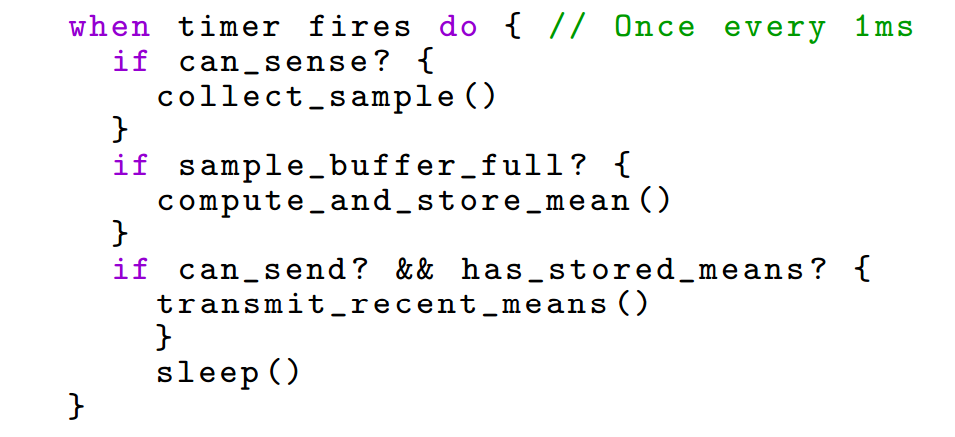
\includegraphics[width=0.99\columnwidth]{figs/listing}
  \caption{{\bf Example program for sensing and sending data}}
  \label{fig:copy}
\end{figure}

The wireless sensor networks community has explored multiple approaches for handling
multitasking on resource limited devices. The designs tend to provide a combination of
timer and event driven context switching as well as a simple programming interface.
TinyOS uses a simple FIFO scheduler to handle event based context switches~\cite{tiny}.
Nano-RK implements priority based preemptive multitasking where task priorities are
statically defined~\cite{nano}. Contiki uses proto-theads, stackless program threads, to
offer a model between Nano-RK and tinyOS. The Contiki implements "cooperative
multithreading" such that events can trigger a context switch, but multithreading may also
be timer based~\cite{contiki}. The goal of multitasking interfaces in wireless sensor
networks is to provide a tradeoff between network lifetime and quality of service. This
differs from the intermittent programming model where the challenge is not system
lifetime, but system functionality based on energy availability.

\section{Chain Discussion}
\chain, while providing a reasonable interface for programmers to work within,
has several inefficiencies that give poor performance on certain applications.
First, there is no notion of data sharing between tasks - all communication is
strictly done through channels. This is useful, as the programmer never needs
to reason about idempotence with respect to their data, but all data that needs
to be transferred between tasks needs to be housed in a channel. Since, under
the original constraints of \chain, channels cannot be written or read from by
tasks that do not own the channel - only tasks that own the channel can access
the data within. This means that large data structures, arrays for instance,
that need to be shared between several channels must be unnecessarily
duplicated in non-volatile memory - one copy of the data structure for each
channel that it needs to be accessed in. Granted, there is no enforcement of
channel ownership by the compiler, but the programmer risks idempotence
violations by straying outside the constraints of chain. We exploit this to
create an equivalent to the multicast-in and multicast-out channels described
in \chain, but using them requires much more reasoning on the part of the programmer.


Additionally, since dynamic memory allocation is arguably too expensive to run
on intermittently powered systems, memory is allocated at compile time.
Unfortunately, since there isn't a compiler specifically for \chain, arrays
are statically sized based on \texttt{\#define} parameters. This can be
create tricky memory corruption errors for the programmer when out-of-bounds
array accesses occur because, for instance, a self-channel has more dirty
fields than \texttt{MAX\_NUM\_DIRTY\_FIELDS}.


\chain also struggles with long-range control flow. For each transition to a
new task, the transition is an explicit one-to-one mapping. \chain provides no
semantics, for instance, to transfer control from task A to task B, then also
transfer control to task C after task B completes, without the programmer
placing \texttt{TRANSITION\_TO(task\_C)} inside task B. This could be done by
using channels in a similar manner to function pointers, while staying within
the semantics of \chain (as we did), but reasoning about code becomes more
challenging for the programmer.


Future work for \chain needs to include some sort of memory allocation based on
the set of channels allocated in the program, but this is work for a compiler
and beyond the scope of this work. For our purposes of threaded applications,
however, \chain is a sufficient launching pad, despite its misgivings since it
does not require specialized hardware or energy subsystems to work effectively,
and since it solves the issue of idempotent data accesses in a way that is
abstracted from the programmer.


\section{System Implementation}
TAPIR has a round robin scheduling algorithm. At the end of a task, the compiler
inserts a jump back to the scheduler task, where the next task in the list is
the one to be executed. An alternate scheduling model that was considered was
a context switch on reboot instead of at the end of each task. The main drawback
of using a reboot-based scheduler is that, because power failure is the common
case, there is a high chance of reducing or halting forward progress altogether
because one thread holds a lock that all of the other threads need but cannot
complete. For that reason the design specifies end of task, so each task has
an opportunity to use a shared resource and release any locks before a power-
intensive context switch occurs. Additionally, a round robin scheduler was
chosen for this design because it is simple to implement and uses only one index counter,
very little power or memory overhead as compared to other scheduling algorithms. It is
critical for multithreading in Chain to not add significant power and memory
overhead in scheduling over conventional Chain so that the workload can
make as much forward progress as possible on one charge cycle. While out of
scope for this project, future work may include a priority scheduler to decrease
latency for certain threads due to context switching for I/O or other input latency
sensitive workloads.

When designing threading in Chain, the shared memory model is a main indicator
of the threaded execution model. The two most probable options when designing
TAPIR were a SIMD execution model of \textit{Thread Pools}, or a MIMD
traditional multiprogramming model. The Thread Pool design makes use of task
code duplication by explicitly forking a number of chain programs, all of which
run simultaneously on the scheduler on arrayed data. This option is useful
multiple data streams from I/O in embedded applications that need to be
processed before new data overrides the I/O device. Additionally, the Thread
Pool model makes sharing memory more regular by using multiple copies of the
same thread. However, this option is not as general purpose. The TAPIR design
ultimately settled on a multiprogramming model, because this allows for the
programmer to explicitly program unique chain programs with shared or discrete
data structures on the same system. However, this execution model requires a
more structured locking mechanism to avoid RMW during execution.

SIMD execution on an intermittent system relies on nonvolatile memory instead
of independent registers for each thread. In Chain's case the implementation
would rely on channels for each thread running in the system. In the MIMD
execution model channels could potentially be re-assigned to already allocated
channels because the threads may end at interleaving times. However, in the
SIMD model it is expected that each identical thread is at a comparable point
in execution to the other running threads, and so each thread that may be
run necessitates a new channel allocation. This could lead to an unavoidable
hard limit on the number of threads that can run in an application which in
turn limits potential applications that are useful on this intermittent device.


\subsection{Scheduler}
For a multi-threaded programming model to exist, one must create a structure to
switch between multiple threads. To keep with \chain's model, we chose to make
the scheduler its own task. The alternative is possible, but since our
implementation of the scheduler required multicast channels, it makes more
sense to have the multicast channels have one endpoint well defined, instead of
some sort of all-to-all channel (which is just a global location in
non-volatile memory). The multicast channels channels are not strictly
necessary, but, all in all, we believe that keeping the scheduler as an
explicit task is good for abstraction. Additionally, if a task has few
self-channels and the data structures passed in those self-channels are
relatively small, the overhead of transitioning to that task is relatively
small, as few double-buffers for self-channels need to be flipped (which is
arguably the largest overhead).


\subsection{Programming Model}
Threaded applications that use POSIX or some other standard library interface
tend to use function calls to interact with the library - for instance, the
user calls a function \texttt{thread\_create} to spawn off a thread.
Unfortunately, this is a difficult programming model to keep under
intermittence, since function calls like \texttt{thread\_create} tend to
involve non-idempotent actions, like appending to a list or incrementing a
variable's value. This leaves two clear options - making the functions to
interact with our threading library \chain tasks, or adding infrastructure to
to our threading library to make the non-idempotent actions that need to occur
act idempotently. We opted for the latter - we feel that it is more valuable to
maintain programmability by provide the user with an interface that they
expect, instead of trying to extend a \chain semantic like
\texttt{TRANSITION\_TO} to also include thread creation.


\subsection{Locking Primitive}
To improve a programmer's control of shared data between threads, and to reduce
the complexity of accessing data that may be touched by many different tasks we
implement a simple mutex object that can be added to a channel. The mutex is
designed to be used in a standard \texttt{channel}, not a double buffered
\texttt{self\_channel}, so it must be able to tolerate a failure after a
read/write operation (i.e. test and set). To achieve idempotence, we add a
\texttt{thread\_id} to the \texttt{free} bit inside of each mutex. When
attempting to acquire a lock, a thread checks if its thread id is equal to the
lock holder, then it checks if the lock is free. If either condition is true,
the thread successfully acquires the lock, otherwise the \texttt{mutex\_lock}
function fails. Upon successfully acquiring the lock, a thread writes its id to
the mutex's holder id, and changes the \texttt{free} bit to \texttt{status =
held}. This scheme guarantees correctness because if a failure occurs after the
mutex is set but before the task commits, the task will read out the id of the
mutex holder before checking if it is free. Upon matching its id with the holder
id, the task will proceed regardless of the fact that \texttt{status = held}.
%TODO Maybe add a figure here to make the sequence of read/write/failure clearer...
Further, a task must finish executing before switching to another thread, so
there is no possibility for an external thread to see a value that was not
committed by another task.


It is important to note that the mutex object can be modified idempotently, but
accesses to the data in the same channel as the mutex must adhere to channel
exclusion. In our example application, the mutex is contained within a user
defined \texttt{shared\_channel} structure that is analogous to a
\texttt{multicast\_channel} but abandons the naming convention that "restricts"
the channel to a static subset of tasks. Any task may read {\em or} or write to
the \texttt{shared\_channel}, but performing both would break correctness. In
the future, a compiler could be used to guarantee that a
\texttt{shared\_channel} is not read and written by the same task, but at
present we believe that the \texttt{mutex} and \texttt{shared\_channel}
interface is easier for programmers to use than \texttt{multicast\_channels}, or
a specialized double buffered channel when passing data between threads. It
maintains familiar semantics for programmers and does not incur the memory
overhead of double buffering.


\subsection{Interrupts}
\subsubsection{Motivation}
Ideally, multithreading would extend to a programming model that can utilize
interrupts in a producer/consumer fashion (i.e. a thread is waiting on data
from an external source, the external source fires an interrupt, the thread
samples the external source and stores the received data in a buffer, and
the thread returns to its original task). However, the inherent
non-deterministic
nature of interrupts from, say, an ADC, creates additional complexity for the
programmer when reasoning about shared memory, especially with respect to
idempotence.


    Specific to the MSP430 architecture (but common in other systems), there is
also the issue of stack integrity. On the MSP430, when an interrupt fires,
the program counter and status register are pushed onto the stack for
the handler to be able to return back to the state of the machine when the
interrupt fired. In our case, however, where power failure is the common
case, an application could experience failure while inside an interrupt
handler. This raises two issues. First, upon reboot from a power failure,
the stack will be cleared (since the stack is stored in volatile memory) and
execution will return to the handler, if we assume that the interrupt handler
is a \chain task. Upon leaving the interrupt, via the MSP430 RETI instruction),
the program's behavior will be undefined. Second, if the programmer does not
use a \chain task for the interrupt handler, it is possible that the interrupt
could fire when the system has a low amount of energy remaining, thus
rendering the system unable to finish executing the interrupt handler,
leading to a host of potential problems.


\subsubsection{Interface}
We provide the functions and macros in figure 3 as an interface to
the programmer. The standard workflow is as follows: the programmer
designates the task that should be run on an interrupt firing
with \texttt{INTERRUPT\_TASK(val, func)} where \texttt{val} is the task
index and \texttt{func} is the function that will be called upon an
interrupt firing - \texttt{val} and \texttt{func} follow the same
interface as \chain tasks. Since we assume that the handler is not
reentrant, the programmer replaces calls to \texttt{\_\_enable\_interrupt()}
with our function \texttt{enable\_interrupts()}.
The programmer's code remains unmodified, with the exception of a call to
\texttt{int\_setup\_complete()} when the \chain program has finished whatever
register initialization is necessary to setup the interrupts for the
application.\\


\begin{figure*}
\begin{minipage}[b]{1.0\textwidth}
\begin{lstlisting}[language=C]
    /** Enable interrupts if int_setup_complete() has been called
      * and execution is not inside an interrupt handler */
    void enable_interrupts();

    /** To be called when setup for the interrupt handler is complete,
      * also enables interrupts */
    void int_setup_complete();

    /** Return from the interrupt handler */
    void return_from_interrupt();

    /** Designate a task to run when an interrupt fires */
    INTERRUPT_TASK(val, func)
\end{lstlisting}
\caption{Interrupt Handling Interface}\label{label-a}
\end{minipage}\hfill
\end{figure*}

\subsubsection{Design}
Working within the constraints of \chain and our multi-programming extensions,
we work to provide a layer of abstraction to the programmer through the standard
layer of tasks and channels. Notably, this includes interrupt handlers being
tasks, rather than standard functions. The alternative has been explored
by keeping specific capacitors for interrupt handlers\cite{Aware}, but this
approach fails if interrupt handlers take longer than the capacitor has
energy for. This bug handlers not completing due to power failure is
unintuitive for programmers coming from consistently powered devices and
makes certain devices unusable under intermittent power.


With interrupt handlers as tasks, if a power failure occurs during a
handler, execution will resume at the handler. This isn't ideal, the
standard paradigm that interrupt handlers are generally short and fast
so that interrupts won't be missed (for instance, a timer interrupt
being missed because processing the interrupt took longer than the
timer period), but we argue that it is more unreasonable to say
that interrupt handlers that take too long will not complete than
to violate the standard paradigm, since the former arbitrarily restricts
the application domain.

\begin{figure}[ht]
\begin{minipage}[b]{.9\columnwidth}
  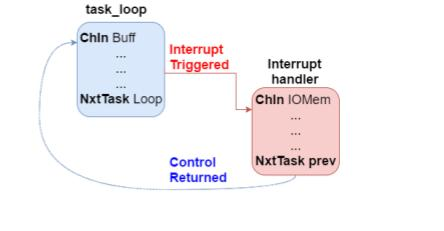
\includegraphics[width=0.7\columnwidth]{figs/int_ctrl_flow}
  \caption{Interrupt Control Flow}\label{intCtrlFlow}
\end{minipage}
\end{figure}

For the sake of simplicity, we assume that interrupt handlers are not
reentrant. Since reentrant handlers can be used in a non-reentrant fashion
without consequences, this assumption does not restrict the application domain.
Moreover, the benefit to reentrant handlers, the application will not miss an
interrupt firing because processing the previous one took too long, is
secondary on intermittent architectures - there is likely a higher chance that
a power failure will occur than an interrupt handler causing an interrupt to be
missed, unless interrupts are firing on an extremely fine granularity.


When an interrupt handler has completed, the programmer calls
\texttt{return\_from\_interrupt()}, which returns execution to the start
of the task that was running when the interrupt occurred. This contradicts
expected behavior - on continuously powered systems, execution generally
returns to the instruction after the instruction that the system received an
interrupt while processing. The continuous system model is intuitive, but
breaks under \chain's intermittence. Task idempotence in \chain only works
when execution returns to the top of a task upon power failure. Program state
(registers and stack memory) are stored
in volatile memory, if an interrupt handler returned to the middle of a task,
it would be impossible to reason about program correctness, since none of the
program state had been stored. The programmer could store program state on the
stack at the start of interrupt handlers, but this would be lost on power
failure. She could also store this program state in non-volatile memory -
trivial for the register set, but difficult and potentially extremely costly to
store the stack, as execution could be several functions deep. Even determining
how much stack to save could be prohibitively costly. Another alternative would
be to store program state in non-volatile, but this has been shown to be
prohibitively costly in most applications \cite{Aware}.


\section{Implementation}
\subsection{Scheduler}

The data structures for our scheduler are listed in figure \ref{schDataStruct}.
Like the rest of chain, memory for data structures is allocated at compile
time. Thus, the limit on the maximum number of threads allowed in a system is
fixed arbitrarily - not ideal, but there isn't a better option while operating
inside chain. The \texttt{threads} array is stored in all-to-one channel, from
every task to the scheduler task. The \texttt{free\_indices} array is stored
in a one-to-all channel, from the scheduler task to every task.


Neither all-to-one nor one-to-all channels fit into standard \chain channel
semantics, although they resemble multicast-in and multicast-out channels
described in the original \chain paper. We eschew the notion that channels
have fixed start and end points and instead treat the channel as a general
location in non-volatile memory that can be read from and written to by
arbitrary tasks. However, accesses to these channels are encapsulated by our
library, so the programmer has no need to think about idempotency violations.


With these multicast channels, the scheduler task can act as a buffer between
multiple threads - arbitrary tasks write \texttt{threads[]} with calls to
\texttt{thread\_create} and \texttt{thread\_end} and tasks read from
\texttt{free\_indices} through calls to thread create, maintaining
idempotency. Inside the scheduler task, we read and write \texttt{current},
so \texttt{current} is double buffered. The only issue is with
\texttt{thread\_init} since it is called from user-defined tasks and
initializes \texttt{current} - the same task that called \texttt{thread\_init}
could call \texttt{thread\_create}, and the \texttt{thread\_create} call
wouldn't see the update to the variable. Since \texttt{current} is always
initialized to the same value (0), we opt for manually swapping the buffer on
\texttt{current} so that other threads can see the update.

\begin{figure}[ht]
\begin{minipage}[b]{.9\columnwidth}
\begin{lstlisting}[language=C]
    typedef struct thread_t {
        unsigned thread_id;
        context_t context;
    } thread_t;

    typedef struct thread_state_t {
        thread_t thread;
        unsigned active;
    } thread_state_t;

    // Array of running threads
    thread_state_t threads[MAX_NUM_THREADS];

    // List of free indices in threads[]
    unsigned free_indices[MAX_NUM_THREADS];
    unsigned free_indices_size;

    // Index of current running thread
    // Stored in self channel
    unsigned current;
\end{lstlisting}
\caption{Scheduler Data Structures}\label{schDataStruct}
\end{minipage}
\end{figure}

We keep an unsigned integer, \texttt{curr\_free\_index}, in volatile memory,
zeroed on every reboot, that acts as a current pointer in
\texttt{free\_indices[]}. Every time the scheduler task runs,
\texttt{free\_indices[]} is updated with the state of \texttt{threads[]},
based on whether or not the active bit is set for a given index. When
\texttt{thread\_create} is called, if \texttt{curr\_free\_index} is greater
than \texttt{free\_indices\_size}, then \texttt{thread\_create} will fail in
POSIX fashion - the system does not have enough resources to support another
thread. Otherwise, \texttt{threads[free\_indices[curr\_free\_index]]} is set
to the new thread. Upon power failure, \texttt{curr\_free\_index} is reset to
zero, so as long as the rest of the operations in the task are idempotent, so
will \texttt{thread\_create} calls - the same locations in \texttt{threads[]}
will be overwritten.

\begin{figure}[ht]
\begin{minipage}[b]{.9\columnwidth}
  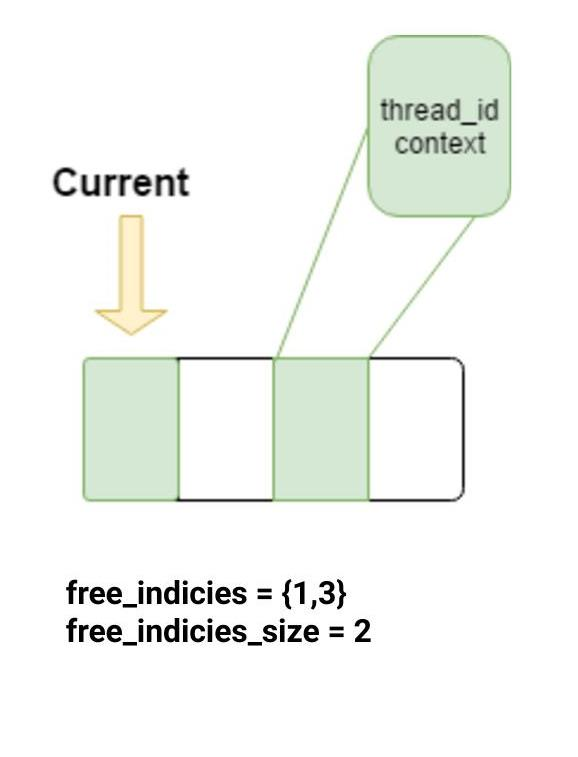
\includegraphics[width=0.7\columnwidth]{figs/threadsArray}
  \caption{Threads Array}\label{threadsArray}
\end{minipage}
\end{figure}


\subsection{Interrupts}
The primary issue with interrupts is the interrupt enable flags. The MSP430,
like many other embedded architectures has a master interrupt enable,
as well as specific, device-level interrupt enables. Both are the user's
responsibility, and need to be specified in the user-defined
\texttt{INIT\_FUNC}, as both will be cleared on reset. When an interrupt fires,
however, interrupts will be disabled by the CPU (again, on most architectures)
and if the device loses power immediately after an interrupt occurs, there will
be no record that the interrupt occurred. This case is unavoidable on
intermittent power without explicit support from the power system - we reason
that if the user cared about every interrupt that fired and if missing one
interrupt would be catastrophic to the device's operation, then, arguably, that
device should not be intermittently powered.


Beyond this, there remains the issue of how to return to the interrupt task
with the interrupt enable set to the correct value if a power failure occurs.
Since interrupts are disabled on boot (on the MSP430, for instance), the user
needs to add code to their \texttt{INIT\_FUNC} to enable interrupts. However,
since interrupt handlers are assumed to be non-reentrant on our system, if
we are inside an interrupt handler, we need to keep interrupts disabled. We
also need to write the address of the task that we should return to upon boot -
the address of the \texttt{INTERRUPT\_TASK} on our system. If these are two
separate variables, there is a correctness issue with respect to power
failures. If we write the location of the \texttt{INTERRUPT\_TASK}, but die
before we can write the fact that we are in an interrupt handler, we will
return to the interrupt handler with interrupts enabled (since they will be
enabled by the \texttt{INIT\_TASK}. If we reverse the order and write the fact
that we are in an interrupt handler, then die before we can write the address
of the \texttt{INTERRUPT\_TASK}, we will resume execution at a non-interrupt
task with interrupts disabled, since the \texttt{INIT\_TASK} will not re-enable
them. Both of these cases could cause execution to fail; the former fails if
the interrupt handler is not written to be reentrant, the latter fails since
interrupts will never be processed. Thus, these writes need to be atomic.


We could depend on the programmer to designate all tasks that would be run as
part of the interrupt handler, then use whether the current task address was
equivalent to one of those as the flag that designates that we are in an
interrupt handler, but this forces tasks to either be used as a part of the
interrupt handler or not, which is bad for code reuse. This also prevents the
user from being able to spawn off non-interrupt tasks as part of an interrupt
handler.


Instead, we exploit the fact that, generally, architectures are byte-aligned
with a fixed instruction size of 16 bits or more - this means, at the very
least, the lowest bit of any code address is zero. As this is true of ARM,
RISC-V, MSP430, and most RISC architectures, we feel that this is a reasonable
assumption. We use this fact to store the flag that is set if execution is
inside an interrupt handler in the lowest bit of the address of the task that
we are currently executing (the task that execution will return to upon
reboot). Thus, we can use a single write to encode all the needed information,
giving atomicity. For simplicity for the programmer, upon an interrupt firing,
an \texttt{interrupt\_prologue()} is run that does this write. The address stored
in the current context is still the address of the user-defined
\texttt{INTERRUPT\_TASK}. In our model, this write is the guarantee that the
system has received the interrupt - if power fails between when the interrupt
fires and this write occurs, the interrupt will be ignored. This could be fixed
by having a special capacitor in the power system to accommodate the write, but
assumptions about the power system, arguably, should not be a part of \chain.


To avoid the pathological stack corruption case described in the motivation for
interrupts, we keep a flag in non-volatile memory that is set if a reboot has
occurred while in an interrupt handler and is unset otherwise. This flag is
unset in the aforementioned \texttt{interrupt\_prologue()} and set in
\texttt{main()}. If and only if the flag is unset when
\texttt{return\_from\_interrupt()} is called, the two values pushed on the
stack from an interrupt firing are popped off. Otherwise the stack remains
unchanged, since the values will have been effectively cleared by a power
failure.


As of this writing, interrupts are still being debugged, but the above
reasoning seems, in theory, correct.
% TODO Mutexes (Simple, meant for pseudo channels) - Emily\\


\section{Evaluation}
To test our multithreading library and mutex implementation, we instrumented
several existing Chain applications that do not share any tasks or channels to
run concurrently. The programs were run on either an MSP430FR5949 launchpad or
on a Capybara sensing node, a custom intermittent development board with an
MSP430FR5949 MCU. Reboot tests were carried out strictly on the Capybara board
because was simpler to guarantee the isolation of the MCU from the programming
FET than on the launchpad. We did not seek to fully verify our implementation
of multi-threading, but we use our experience in application development to
support our claim that the threads behave correctly, and as a programmer would
expect.

\subsection{Applications}
\subsubsection{Blinker (B)}
This application was built on top of the app-blinker-chain
example~\cite{blinker} and modified to remove the delays and LED activations, so
that it just passes data through three tasks until a maximum count is reached,
and then the thread terminates. This app was used to demonstrate the
initial functionality of the system, and then to test mutexes. In both cases a
combination of \texttt{LOG} statements and final output values were used to
confirm the correct operation of the system, however we do not report memory
usage or reboots during execution for this application. 
\subsubsection{Cuckoo-RSA (CRSA)}
This application is a combination of a cuckoo filter that inserts and queries 64
values a Bloom filter-like data structure~\cite{Chain}, and RSA encryption of message
using 128-bit keys~\cite{Chain}. Unfortunately this is the only application
combination where merging the original applications did not produce the same
final result as running the applications separately. Several bytes at the end of
a crucial array for RSA were always overwritten when the applications were
merged, and we were unable to fix the problem. Unit tests running the RSA
application in single threaded mode through our scheduler and using our
multi-threading library produce the correct result, but any combination of RSA
and cuckoo filtering produces the incorrect result. However, RSA does run to
completion, so we believe at least the memory overhead results from C-RSA are still useful.
\subsubsection{Cuckoo-Bitcount (CB)}
This application is a combination of the cuckoo filter described above and a
application that uses different algorithms to count the number of bits in an
array of integers~\cite{bitcount}. CB is a correctly working combination of two
applications that produces the same output as separate executions of the
unmodified versions of these applications. It expands the reliability of our
multi-threading library beyond simple applications like Blinker.
\subsubsection{Cuckoo-Bitcount-Blinker(CBB)}
CBB combines the cuckoo filter and bit count applications with two threads of
the blinker application. This results in four active threads at once, which is
the maximum number of threads our prototype implementation allows. We confirmed
that all four threads are fairly serviced by the round robin scheduler and they
correctly start and end.

\subsection{Results}
CRSA, CB, and CBB were ported from multithreaded applications to serial
applications. Rather than using the scheduler to switch between tasks, the an
application transitions to the first task of the successive application upon
completion. The memory overhead of RSA and Bitcount when they are instrumented
to run as a single thread with the additional overhead of the scheduler is shown
to provide a reference for the baseline cost of the scheduler.
Figure~\ref{fig:mem} shows the increase in code size with the switcht to the
multithreading library. Approximately 3 lines or code in user space needed to be
added to each of the multithreaded applications, but the library code is
significant. The fraction of overhead ranges from 12.6\% for CB to nearly 30\%
for bitcount.  

\begin{figure}[h]
  \centering
  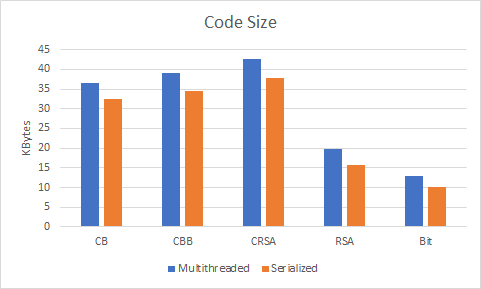
\includegraphics[width=0.99\columnwidth]{figs/memory}
  \caption{{\bf Increase in code size}}
  \label{fig:copy}
\end{figure}

We measure the performance of the application in terms of the number of reboots
that occur before the application completes. This is an accurate measurement of
performanc in intermittent systems because the majority of the execution time is
spent recharging the capacitors. In our system set up, as shown in Figure
~\ref{fig:setup}, the capacitor charging time is consistent at approximately 3.5
seconds. We only report reboot data for CBB and CB because of the discrepancy in
CRSA output between the multithreaded and serial versions.
Figure~\ref{fig:reboots} shows that the scheduler has a significant cost to the
system. The multithreaded executions incur significantly more reboots than the
serial versions. This is to be expected due to the additional instructions of
scheduler code and additional writes to non-volatile memory required to access
the scheduler. 
\begin{figure}[h]
  \centering
  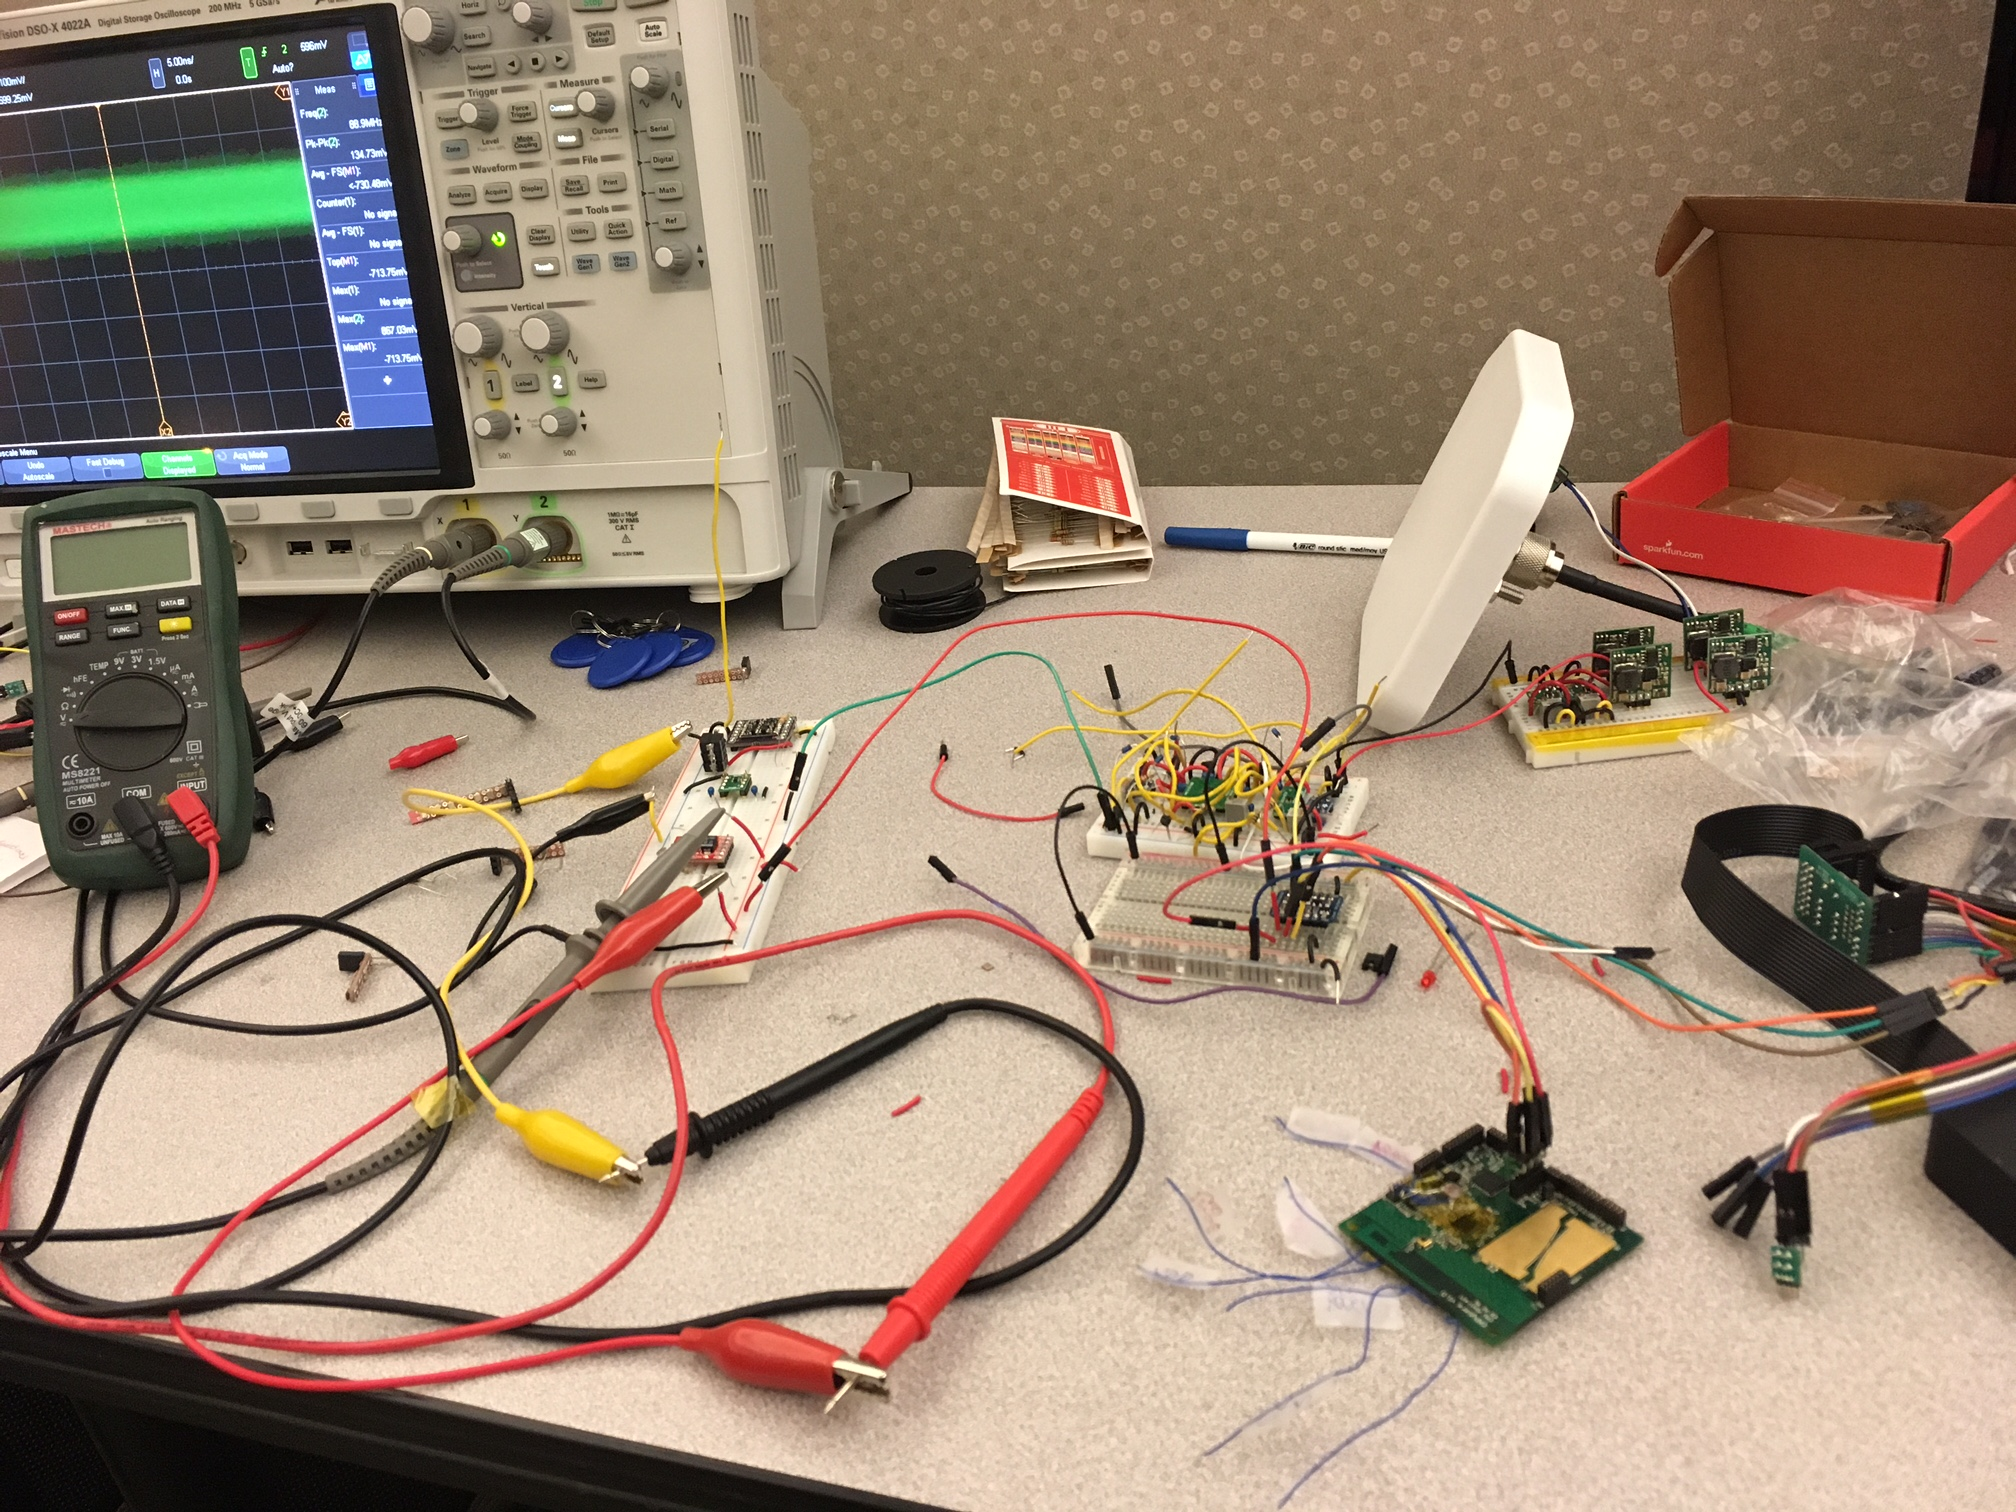
\includegraphics[width=0.99\columnwidth]{figs/setup}
  \caption{{\bf Test setup using a Capybara board, and RF power source}}
  \label{fig:setup}
\end{figure}

\begin{figure}[h]
  \centering
  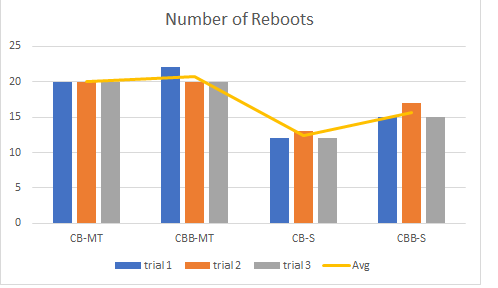
\includegraphics[width=0.99\columnwidth]{figs/reboots}
  \caption{{\bf Number of reboots per execution}}
  \label{fig:reboots}
\end{figure}


\section{Future Work}
Future work is focused on saving memory by using channel and code reuse
optimizations when forking new chain programs from current tasks.  When forking
a new task, a channel may be duplicated, which linearly increases the amount of
memory necessary for channels with the number of currently running programs.  It
is possible to reuse channels between tasks if the number of iterations of that
task are known at compile time and it can be estimated how many are to be
running simultaneously. A register allocation graph coloring scheme can then be
repurposed for reusing channels allocated at compile time.  In either case the
current channel naming scheme must be changed to support channel duplication,
ether real or simulated.  Currently channels are allocated and named at compile
time by combining the names of the input and output channel tasks.  However, if
tasks can be duplicated this naming scheme must be altered to support multiple
channels of the same name and potentially multiple channels of the same name.
This can be done with a vector clock timestamp or a simple counter stored in
nonvolatile memory to create unique channel names.

Additionally, it is possible to save memory by sharing arrays between tasks
without the necessity of copying the array in its entirety in each channel.  To
do this the concept of intermittent tasks mutexes for shared resources and data
structures would be introduced.  The structures are protected by a lock that
contains the thread ID of the task that currently holds the lock.  In order to
allow all tasks access to a data structure without breaking all chain semantics,
a modified version of a module channel would be used in order for multiple tasks
to potentially modify one channel.  However, even with that change it is
challenging to define sharing between threads in an intermittent context and to
maintain chain semantics while implementing shared data structures while still
maintaining correctness.  Because channel sizes are constrained at compile time
currently, it is also necessary to know at compile time all data structures,
shared or private, that are going to be used during execution of a chain program
or programs.  It is a challenge for future work in this field to constrain
memory for channels at compile time and for the compiler to know with certainty
how much memory is necessary to allocate. Depending on the workload, the amount
of forked threads would need to be constrained such that threads don't overflow
nonvolatile memory at runtime.

Future work also includes optimizations to reduce overhead, such as converting
the free indices array to a free indices bitmap in order to reduce the amount of
baseline memory that the scheduler task uses.  Re-assignation and re-use of
channels at runtime would increase overhead, but it is thought that the memory
saved by this procedure is worth the trade-off of increased overhead.  If
re-assignation can be determined at compile-time, the overhead during runtime
will still remain low.

\section{Conclusion}
The increased prevalence of IoT devices necessitates an increased ability to
run larger, general purpose applications on devices with smaller memory and
energy footprints. With the increased research on intermittently powered devices
for use in the embedded sphere, it is a logical next step to explore the use
of general purpose threaded code on an intermittent device. We have shown
through the design and implementation of TAPIR on top of the Chain intermittent
programming model that adding functionality for multiprogramming with
multithreaded applications can have a low enough memory and power overhead to be
considered useful on such a device. Additionally, we have implemented a safe
locking structure for use in nonvolatile memory for such applications that
maintains RMW restrictions in the intermittent execution model and allows
for larger shared data structures without the overhead of memory duplication
that may overcrowd a small device. We have shown with this design that threaded
applications can be programmed in a familiar way to software designers and that
it is a viable next step in intermittent device research.

\begin{figure}[h]
  \centering
  
\includegraphics[width=0.9\columnwidth]{figs/tapir}
\end{figure}


\balance
\bibliographystyle{abbrv}
\bibliography{sigproc}  % sigproc.bib is the name of the Bibliography
\end{document}
